\chapter{Einführung}

\section{Algorithmus, Problem, elementare Schritte}

\subsection*{Algorithmus}
    \begin{itemize}[label={-}]
        \item löst ein bestimmtes Problem
        \item braucht dafür endlich viele Schritte
        \item alle Schritte sind elementar
    \end{itemize}


\subsection*{Problem}
    \begin{itemize}[label={-}]
        \item formal beschrieben: Spezifikation
    \end{itemize}

    \medskip


    \begin{enumerate}
        \item Vorbedingung: in welchem Zustand muss die \glqq Welt\grqq sein, damit der Algorithmus ausgeführt werden kann?
        \begin{itemize}[label={$\rightarrow$}]
            \item falls Vorbedingung nicht erfüllt: Fehlermeldung (nicht stillschweigend falsches Ergebnis)
        \end{itemize}
        \item Nachbedingungen: in welchem Zustand ist die \glqq Welt\grqq nach Ende des Algorithmus
        \begin{itemize}[label={$\rightarrow$}]
            \item wie kann man feststellen, dass der Algorithmus korrekt durchgelaufen ist?
        \end{itemize}
    \end{enumerate}

    \medskip

    $\underline{\text{Beispiel}}$: $y = \sqrt{x}$ \\
    \begin{itemize}[label={}]
    \item $\underline{\text{Vorbedingungen}}$ :
        \begin{itemize}
            \item $x \in \mathbb{R}$ oder $ x \in \mathbb{N}$
            \item $x \ge 0$
        \end{itemize}
    \item $\underline{\text{Nachbedingung}}$:
        \begin{itemize}
            \item $y * y = y^{2} = x$
        \end{itemize}
    \item $\underline{\text{Varianten}}$:
        \begin{itemize}[label={-}]
            \item falls $x < 0 \rightarrow$ Alg. gibt Fehlermeldung
            \item falls $x < 0 \rightarrow y = NaN$ (``not a number'': spezieller Zahlenwert für genau diesen Zweck, wenn etwas nicht berechnet werden kann) Vorteil: nicht direkt Programmabbruch weil Fehlermeldung
        \end{itemize}
    \end{itemize}




\subsection*{Elementare Schritte}
charakterisieren das Gerät (bzw. Menschen), der den Algorithmus ausführen soll (``Spielregeln'' ) \\

\begin{itemize}[label={–}]
    \item Beispiel: Geometrie mit Zirkel und Lineal (alte Griechen)

        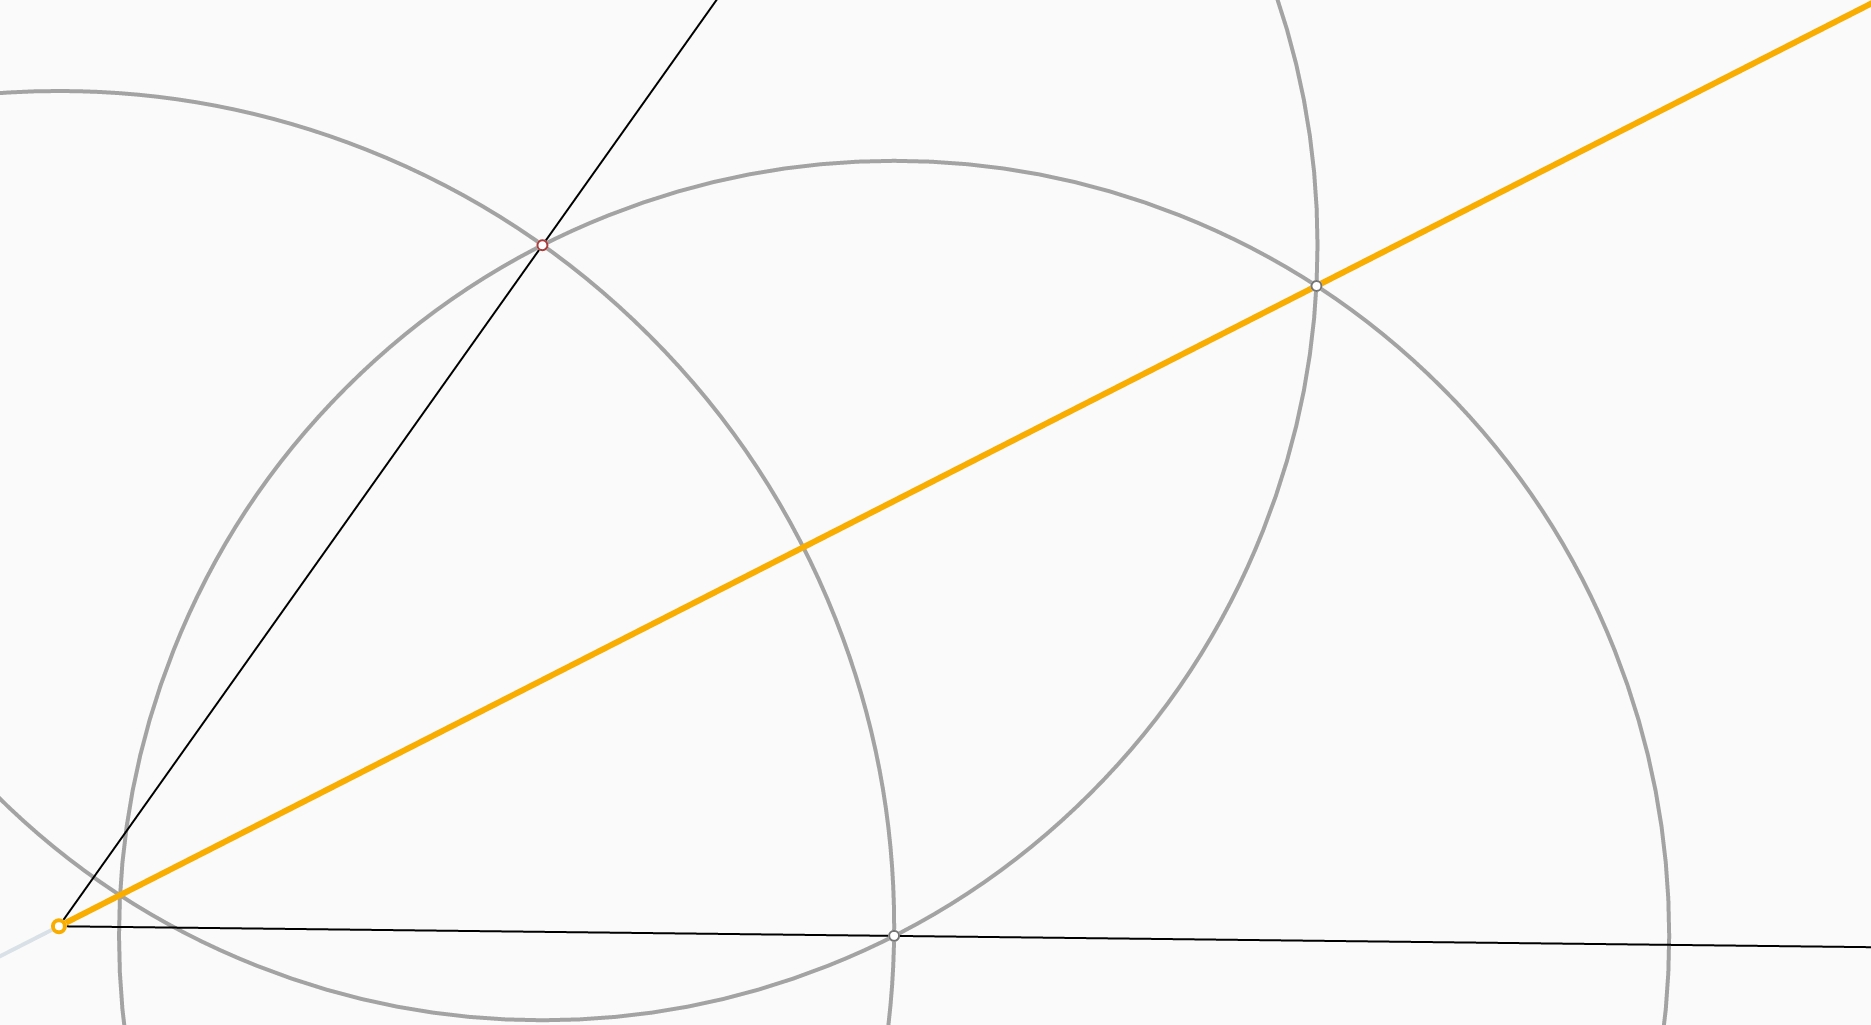
\includegraphics[width=13cm,height=7cm,keepaspectratio]{./Pictures/Winkelhalbierende.png}


    Winkelhalbierende eines Winkels:
    elementare Schritte:
    \begin{enumerate}
        \item einen Punkt definieren (-beliebig oder - Schnittpunkt von Linien)
        \item mit Zirkel Abstand von 2 Punkten abgreifen
        \item mit Zirkel einen Kreis um einen bestimmten Punkt zeichnen
        \item Zwei Punkte mit dem Lineal verbinden
    \end{enumerate}


    \item Abakisten vs. Algorithmiker (1200 bis 1500)
    \begin{itemize}[label={-}]
        \item Abakisten rechnen mit römischen Zahlen und Abakus
        \item Algorithmiker (al Quarismi: Rechnen mit indischen / arabischen Ziffern (ursprünglich aus Indien) schriftliches Rechnen wie in der Grundschule) ~800
        \item ~1200 lateinische Übersetzung ``Dixit $\underline{\text{Algorismi}}$''  $\leftarrow$ Herkunft Wort
        \item Vereinigung um 15000 : Adam Riese (Rechnen auf den Federn und Linien)
    \end{itemize}

    \item $\underline{\text{elementare Schritte im modernen Computer:}}$ \\
    $\begin{rcases}
    \bullet & \lambda\text{-Kalkül} \\
    \bullet & \text{rekursive Funktionen (Gödel)} \\
    \bullet & \text{while-Programme} \\
    \bullet & \text{Turing-Maschinen }
    \end{rcases}$ ganz untersch. Sammlungen von elementaren Schritten
    \bigskip

    $\underline{\text{Aber}}$: die Menge der Algorithmen, die man damit implementieren kann, sind identisch!
    ``$\underline{\text{Menge der berechenbaren Funktionen}}$'' $\rightarrow$ worüber die Informatik spricht



    \item $\underline{\text{while-Programme:}}$ \\
        in verbesserter Form von allen CPUs implementiert
    \begin{itemize}[label={-}]
        \item vier Grundoperationen:
        \begin{itemize}
            \item Addition einer Konstanten : \verb|x[j] = x[i] +c| \\
            \verb|x[j] =| Inhalt der Speicherstelle j; \verb|c =| Konstante
            \item Subtraktion einer Konstanten: \verb|x[j] = x [i] - c| \\
             `` $=$'' $\rightarrow$ Zuweisung
            \item Nacheinanderausführung von Programmen P und Q $\rightarrow$ \verb|P ; Q| (erst \verb|P|, dann \verb|Q|)
            \item Schleife:  \verb|WHILE x[i] != 0 DO P DONE| \\
            Programm \verb|P| sollte \verb|x[i]| irgendwann auf \verb|0| setzen, sonst Endlosschleife $\widehat{=}$ kein Algorithmus
        \end{itemize}
    \end{itemize}


    \item erstaunlicher Fakt: alle berechenbaren Funktionen können mit nur 4 elementaren Operationen ausgedrückt werden: \\
    in Backus-Naur-Notation:


    \begin{minted}{python}
Programm ::= x[i] = x[j] + c                  # Addition einer Konstanten
         |   x[i] = x[j] - c                  # Subtraktion einer Konstanten
         |   Programm ; Programm              # Nacheinanderausfuehren
         |   WHILE x[i] != 0 DO Programm DONE # Wiederholtes Ausfuehren
    \end{minted}


    Beispiel: Addition von zwei Speicherzellen \verb|x[i]| und \verb|x[j]| \\
    Spezifikation des Algorithmus: \\
    \vspace{-12mm}
    \begin{singlespace}
    \begin{itemize}[label={-}]
        \item Vorbedingung: \verb|x[j] >= 0| \\
        \item Nachbedingung: \verb|x[i]' = x[i] + x[j]      (x[i]' = x[i] |am Ende des Alg.\verb|)|
        \item Algorithmus:      \begin{minted}{python}
        WHILE x[j] != 0 DO
        x[i] = x[i] + 1 ;
        x[j] = x[j] - 1
        DONE
                                                \end{minted}
    \end{itemize}
    \end{singlespace}

in der Praxis ist das $\underline{\text{sehr ineffizient}}$: Anzahl der Schritte $\bigO{}(x[j])$ es geht auch mit $\bigO{}(log(x[j]))$ Schritten

    \item[$\Rightarrow$] pragmatische Definition von elementaren Schritten
    \begin{itemize}[label={-}]
        \item Hardware-orientierte Definition: elementare Schritte sind alle Operationen, die die jeweilige CPU anbietet (``Assembler'' ) (``Maschinensprache'' )
        \item Software-orientierte Definition: elementare Schritte sind alle Operationen, die die Programmiersprache, inklusive ihrer Standardbibliothek, anbietet.
    \end{itemize}

\end{itemize}

\section{Was ist eine Datenstruktur?}

\begin{itemize}[label={-}]
    \item Daten sind Folgen von Bits d.h. 0/1 - Folgen \\
    \begin{center}
    $1101,0110,0110,1100$
    \end{center}
    Bitfolgen allein haben $\underline{\text{keine}}$ Bedeutung, man braucht zusätzlich eine Interpretations-Vorschrift $\widehat{=}$ ``Datenformat''
    \item Beispiele:
    \begin{itemize}[label={$\bullet$}]
        \item Interpretation als ``unsigned integer 16'' \\
        \begin{tabular}{C{5mm} C{5mm} C{5mm} C{5mm} C{5mm} C{5mm} C{5mm} C{5mm} C{5mm} C{5mm} C{5mm} C{5mm} C{5mm} C{5mm} C{5mm} C{5mm}}
            1 & 1 & 0 & 1 & 0 & 1 & 1 & 0 & 0 & 1 & 1 & 0 & 1 & 1 & 0 & 0 \\
            $\uparrow$ & $\uparrow$ & $\uparrow$ & $\uparrow$ & $\uparrow$ & $\uparrow$ & $\uparrow$ & $\uparrow$ & $\uparrow$ & $\uparrow$ & $\uparrow$ & $\uparrow$ & $\uparrow$ & $\uparrow$ & $\uparrow$ & $\uparrow$ \\
            $2^{15}$ & $2^{14}$ & $2^{13}$ & $2^{12}$ & $2^{11}$ & $2^{10}$ & $2^{9}$ & $2^{8}$ & $2^{7}$ & $2^{6}$ & $2^{5}$ & $2^{4}$ & $2^{3}$ & $2^{2}$ & $2^{1}$ & $2^{0}$ \\
            =33768 & & ... & & & & & & & & & & & & =2 & =1 \\
        \end{tabular}

        33768 + ... + 8 + 4 + 0 + 0 = 54892
        \item Interpretation als ``signed integer 16 im 2er-Komplement'' \\
        Regel:
        \begin{itemize}[label={-}]
            \item wenn das linke Bit 0 ist $\Rightarrow$ unsigned int 15
            \item wenn das linke Bit 1 ist $\Rightarrow$ negative Zahl
        \end{itemize}
        $ -10644 = \begin{cases}
        \bullet \hspace{1mm} \text{alle Bits negieren und 1 addieren} \Leftrightarrow \text{interpretiere Erg. als ``unsigned int 15''} \\
        0010100110010011 \\
        \underline{\hspace{2,65cm} + 1}\\
        \hspace{2.3mm} 010100110010100
        \end{cases}$

        Ausnahme:  \\
         \hspace*{0.5cm}negieren 0111111111111111 \\
         \hspace*{1.7cm} + $\underline{ \hspace*{2.8cm} 1}$ \\
         \hspace*{2.1cm}1000000000000000 = definiert als $-2^{15}$ \\
         \hspace*{0.5cm}(die Zahl $+2^{15}$ ist in signed int 16 nicht darstellbar)


        \item Interpretation als Windows-Zeichensatz, zwei 8-bit Zeichencodes \\
        \hspace*{3cm} $\underbrace{11010110}_{\text{``Ö''}}  \hspace*{0.5cm} \underbrace{01101100}_{\text{``l''}} \Rightarrow$ Öl

        \item   Interpretation als Gleitkommazahl ``float 16'' nach dem Standard IEEE 754 \\
        \hspace*{3cm} $\underbrace{1}_{\text{sign = s}}  \hspace*{0.5cm} \underbrace{10101}_{\text{exponent = e}} \hspace*{0.5cm} \underbrace{1001101100}_{\text{mantisse = m}} $ \\
        \hspace*{3cm} $z = (1-2*s) * 2^{e-15} * (1 + m * 2^{-10})$ \\
        \hspace*{3.28cm} $= -102.75$

        \item[] usw. (unendlich viele Interpretationen)
        \end{itemize}
    \item wichtig bei Daten in Dateien: Dateien sind Bitfolgen auf Festplatte,
    \item[] $\rightarrow$ man braucht Interpretation:
    \begin{itemize}[label={-}]
        \item nach Ende des Filename: .jpg
        \item im Internet: Mime-types (Multipurpose Internet Mail Extension): mit den Daten verknüpfte Typ-Info
        \item magic numbers am Fileanfang: 255 216 255 (sonst kein .jpg, selbst wenn Endung vorhanden $\rightarrow$ evtl. Virus)
        \item alternative Möglichkeiten, Datenstrukturen zu definieren \\
        \begin{figure}[htbp]
            \begin{minipage}[t]{6cm}
                \vspace{0pt}
                \centering
                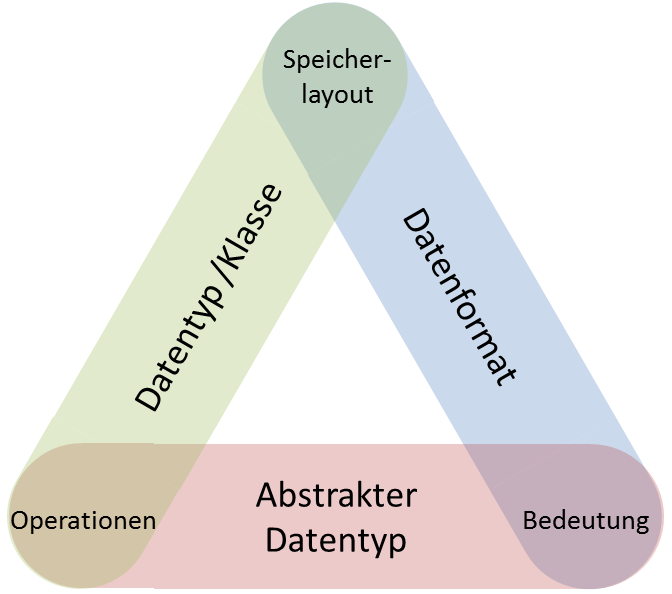
\includegraphics[width=8cm,height=8cm,keepaspectratio]{./Pictures/Dreieck.png}
                \label{fig:Bild1}
            \end{minipage}
            \hfill
            \begin{minipage}[t]{6cm}
                \vspace{0pt}
                Datenformat $\leftarrow$ Files \\
                Datentyp/Klasse $\leftarrow$ Programmiersprache \\
                Speicherlayout = Bitfolge \\
                Operationen = erlaubte Operationen \\
                Bedeutung = Interpretation \\
                String:
                \begin{itemize}[label={-}]
                    \item Bytefolge der Zeichen
                    \item Operationen: print, append, to\_lower\_case
                \end{itemize}

            \end{minipage}
        \end{figure}

        ADT $\widehat{=}$ $\underline{\text{abstract}}$ data type: Datentypen werden definiert, $\underline{\text{ohne}}$ eine spezielle Implementation als Bitfolge \\

        $\Rightarrow$ Theorie, abstrakte Spezifikation von Alg. (Pseudocode) \\
        $\Rightarrow$ Vorteil: Programmierer hat große Freiheiten für Implementation

        \end{itemize}
\end{itemize}

\section{Fundamentale Algorithmen}
stehen für (fast) alle Typen zur Verfügung
\begin{itemize}[label={$\bullet$}]
    \item Konstruktor:
    \begin{enumerate}
        \item weise einer bestimmten Speicherstelle (Bitfolge) eine Interpretation zu
        \item Initialisiere die Bitfolge mit einem festen Anfangswert (oft 0)
    \end{enumerate}
    \item[] Beispiel: in Python heißt der Konstruktor-Algorithmus wie der Datentyp \\
    \begin{minted}{python}
        i = int()       # ganze Zahl
        f = float()     # Gleitkommazahl
        l = list()      # leeres Array
    \end{minted}
    \item[] alternative Konstruktoren für andere Anfangswerte:
    \begin{minted}{python}
        j = int(2)      # ganze Zahl 2 statt 0
        a = [i, j]      # Array mit den Zahlen [0,2]
    \end{minted}

    \item Vergleiche auf Gleichheit und Identität \\
    \begin{tabular}{C{7cm} C{7cm}}
    $\downarrow$ & $\searrow$ \\
    zwei Variablen des gleichen Typs enthalten die gleiche Bitfolge & zwei Bezeichner (= Variablenname) referenzieren die gleiche Variable \\
    $\downarrow$ & $\downarrow$ \\
    $==$ & \verb|is| \\
    Negation: $!=$ & \verb|is not| \\
    \end{tabular}

    $\begin{rcases}
    \text{a} = [1,2] \\
    \text{b} = [1,2]
    \end{rcases}
    \text{``a} == \text{b''}' \text{ist wahr}; \text{``a} != \text{b''} \text{ist falsch} $ \hspace*{0.6cm}
    ``a \verb|is|  b'' ist falsch; ``a \verb|is not| b'' ist wahr \\

    Es gilt stets:
    \begin{itemize}[label={-}]
        \item ``a \verb|is| b'' wahr $\rightarrow$ ``a $== $b'' wahr
        \item ``a \verb|is| a'' und ``a $==$ a'' immer wahr
    \end{itemize}
    \item swap-Operation: Vertauschen der Bitfolgen von zwei Variablen des gleichen Typs \\
    andere Programmiersprachen: swap(a,b) \\
    Python:
    \begin{itemize}[label={}]
        \item Mehrfachzuweisung: a, b = b, a
        \item Beispiel-Verwendung: Sortieren
    \end{itemize}
\end{itemize}


\subsection*{Referenzsemantik vs. Wertsemantik}
    \begin{itemize}[label={-}]
        \item Wofür steht ein Variablenname in einer Programmiersprache?
        \item Was genau bewirkt die Zuweisung an einen Variablennamen?
        \item Analogie:
    \end{itemize}
    \begin{tabular}{C{7cm} C{7cm}}
    Bookmarks im Internet \hspace*{1cm}vs. &  Download einer Seite \\
    $\Downarrow$ & $\Downarrow$ \\
    URL, mit der man eine Seite wieder aufrufen kann & lokale Kopie der Seite
    kann wieder aufgerufen werden \\
    $\underline{\text{aber:}}$ es könnte auch eine neue sein & $\underline{\text{aber:}}$ könnte veraltet sein \\
    & \\
    URL $\widehat{=}$ Referenz auf die Seite (ähnlich der Adresse einer Wohnung) & Kopie \\
    $\widehat{=}$ & $\widehat{=}$ \\
    Referenzsemantik & Wertsemantik \\
     & \\
    $ \underline{\text{Python:}}$ für alle anderen Typen & Zahlen(int, float, boolean, string)\\
    \begin{minted}[breaklines=false, linenos=false]{python}
    i = [1,2]
    j = i           #j=[1,2]
    i = [0] = 3     #i=[3,2] j=[3,2]
    \end{minted}
                                                         &
    \begin{minted}[breaklines=false, linenos=false]{python}
    i=int(2)
    j=i             # j==2
    i=3             # j==2,
    \end{minted}
    \\
    i und j sind nur alternative Namen für die selbe Speicherstelle & i und j verweisen auf verschiedene Speicherstellen \\
    \end{tabular}




\subsection*{Freiheitsgrade bei der Datenstruktur-Definition}

\begin{itemize}[label={$\bullet$}]
    \item Datenformat: u int8 (8 bit, als unsigned integer interpret.)
    \begin{itemize}[label={-}]
        \item Speicher \& Interpretation festgelegt
        \item Operation: Addition: -Funktionsname ``add'', ``plus'', ``+''
        \item Implementation:  \\
        \hspace*{0.5cm}00000001 \\
        \hspace*{0.05cm} + $\underline{ 00000001}$ \\
        \hspace*{0.5cm}00000010\\

        \hspace*{0.5cm}11111111 $\widehat{=}$ 255 \\
        \hspace*{0.05cm} + $\underline{00000001}$ \\
        \hspace*{0.25cm} 100000000 $\widehat{=}$ 256 $\Rightarrow$ 9 bit ?? \\

        \item Konvention:
        \begin{itemize}[label={-}]
            \item es passiert \emph{nichts}, bleibt 255 \\
            Keine gute Idee, z.B. Kommutativität :( \\
            Beispiel: \verb| i = j + k| wenn j und k vertauscht werden: Was bleibt dann erhalten?
            \item Fehlermeldung: ``Zahl zu groß'' \\
            suboptimal, weil es evtl. zu oft zu Programmabbrüchen kommt
            \item Berechnung ``modulo 256'' \\
            $(255+1)mod256 = 0$ \\
            man rechnet zyklisch \\
            funktioniert ebenso im negativen Bereich
            (CPU: Übertrag der letzten Addition wird gelöscht)
        \end{itemize}
    \end{itemize}
\end{itemize}


